For jet events in small systems like proton-proton and proton-ion collisions, there is a hard scattering as well as additional processes that occur within the collisions including multiple parton interactions and radiation from initial or final state partons of the collision.
These processes all contribute to the underlying event of a jet event and need to be subtracted from the final state jet measurements to accurately trace jet measurements back to initial hard scatterings.
To study the underlying event in jet events, we can divide calorimeter geometry into 4 sections in $\phi$ with respect to the hard scattering reference (highest pT particle or jet). 
Figure \ref{fig:UEeventshape} shows the event shape used for underlying event measurements, where the toward region is defined as $|\Delta\phi| < 60^\circ$, the away region is defined as $|\Delta\phi| > 120^\circ$, and the transverse regions are defined as $60^\circ < |\Delta\phi| < 120^\circ$.
Transverse sections should have limited direct influence from hard scattering allowing for direct measurements of the underlying event.

\begin{figure}
    \centering
    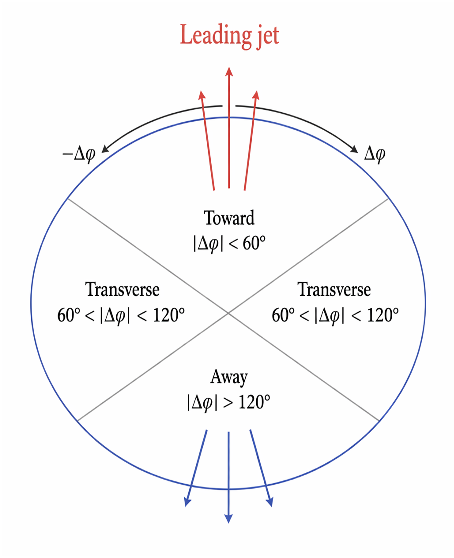
\includegraphics[width=0.5\textwidth]{figures/chapter1/ueeventshape.png}
    \caption{Schematic of event shape used for underlying event measurements.}
    \label{fig:UEeventshape}
\end{figure}

The goal of the analysis in this thesis on the underlying event in p+p collisions is to connect results from underlying event measurements to studies of hard-soft correlations in p+A and p+p collisions at RHIC and the LHC.
Additionally, this thesis seeks to understand the different trends seen in previous measurements of the underlying event at LHC and RHIC, which are event selection dependent at LHC, by connecting to previous explanations of hard-soft correlations in small systems.

\begin{figure}
    \centering
    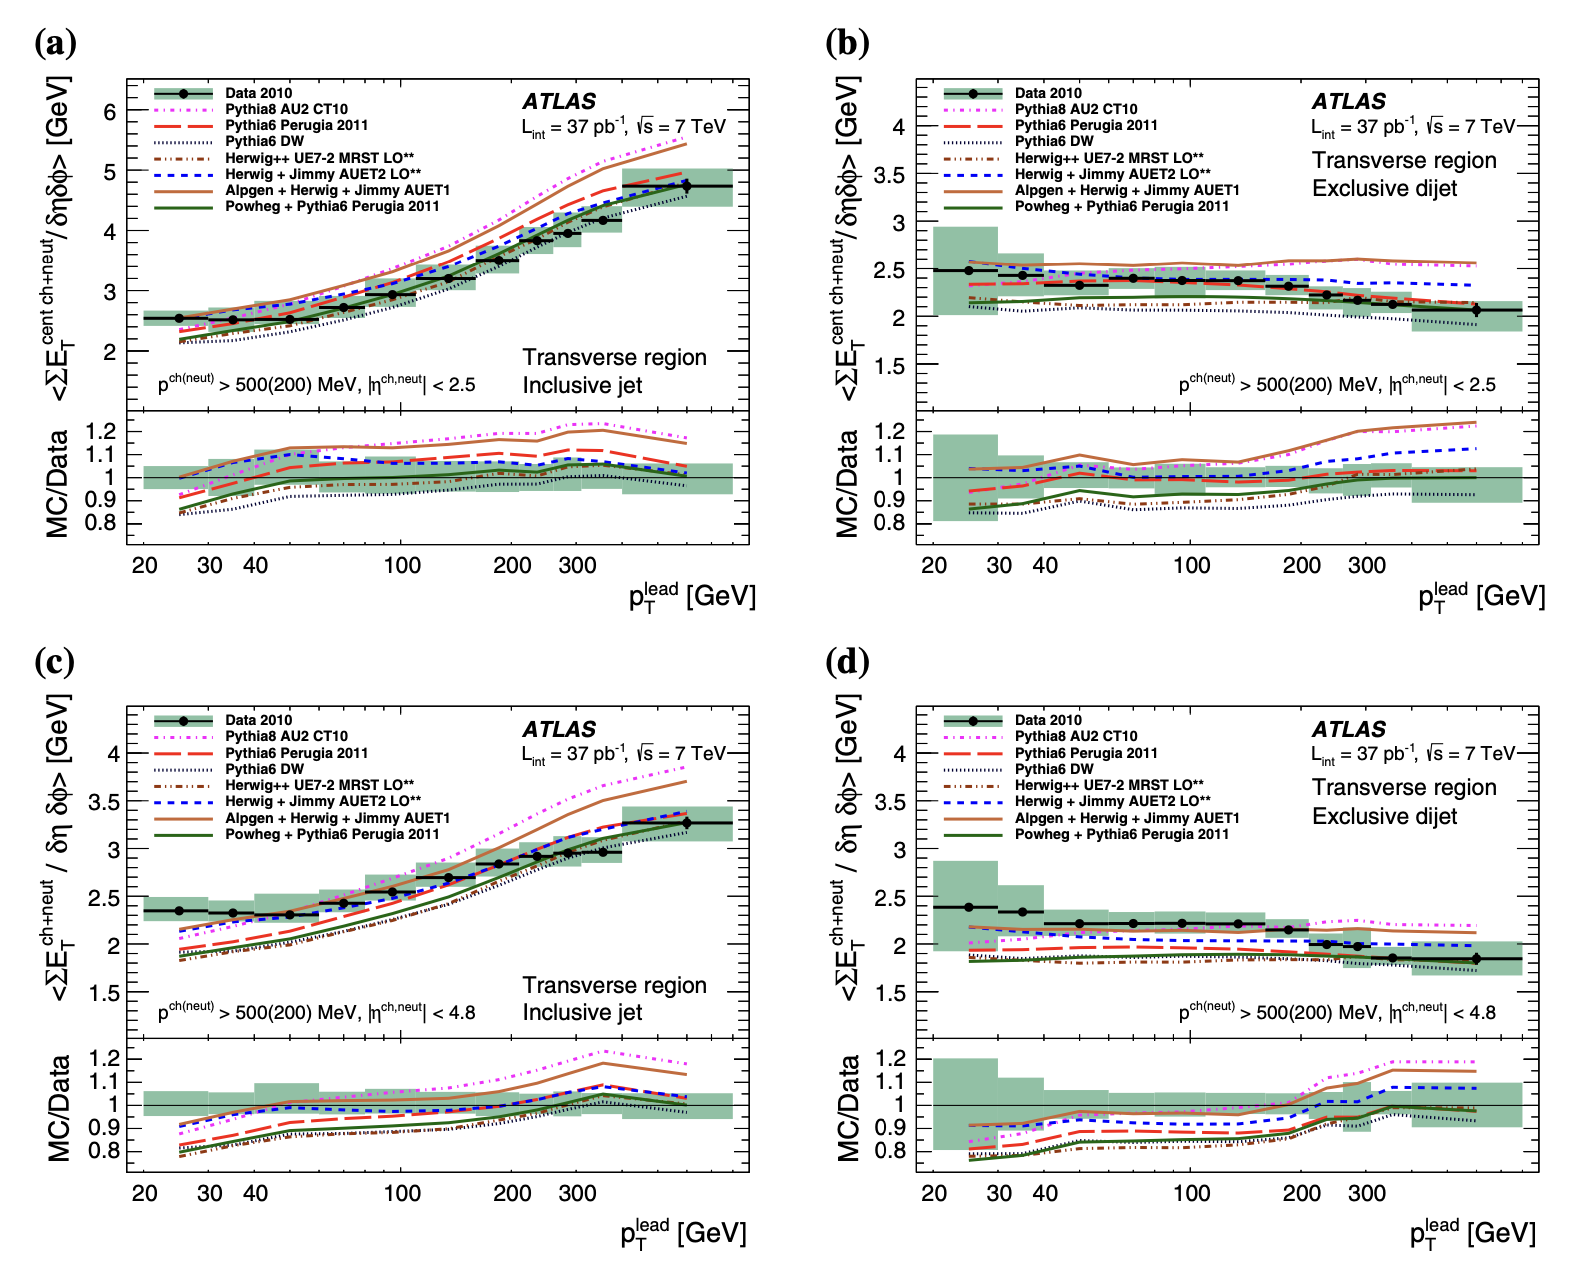
\includegraphics[width=\textwidth]{figures/chapter1/atlas_ue_in_pp_results.png}
    \caption{Underlying event measurements in p+p collisions at 7 TeV from ATLAS. The left plots shows the underlying event as a function of leading jet pT for inclusive jet events, while the right plots shows the underlying event as a function of leading jet pT for exclusive dijet events. Reproduced from~\cite{ATLAS:2014underlying_event_jets_7tev}.}
    \label{fig:ue_pp_atlas}
\end{figure}
At both the LHC and RHIC, the underlying event has been measured in p+p collisions as a function of the leading jet $p_{T}$ using the event shape shown in Figure \ref{fig:UEeventshape}.
Results from the LHC at energies $>1$ TeV show consistent results that the UE rises as a function of leading jet $p_{T}$, which is expected from a simple picture of the underlying event where harder collisions (collisions with higher $Q^2$) have more initial and final state radiation and are more central collisions thereby having more multiple parton interactions.
An example of these results are shown from the ATLAS experiment at 7 TeV~\cite{ATLAS:2014underlying_event_jets_7tev} in Figure~\ref{fig:ue_pp_atlas}.

However, also shown are additional results from ATLAS at 7 TeV using an event selection requirement of back-to-back dijets and no third jet in the event, defined as "exclusive dijet" events, show a different trend.
Here with the exclusive dijet selection, the UE decreases slightly with increasing leading-jet $p_{T}$ which is unexpected in the simple picture of the underlying event. 
\begin{figure}
    \centering
    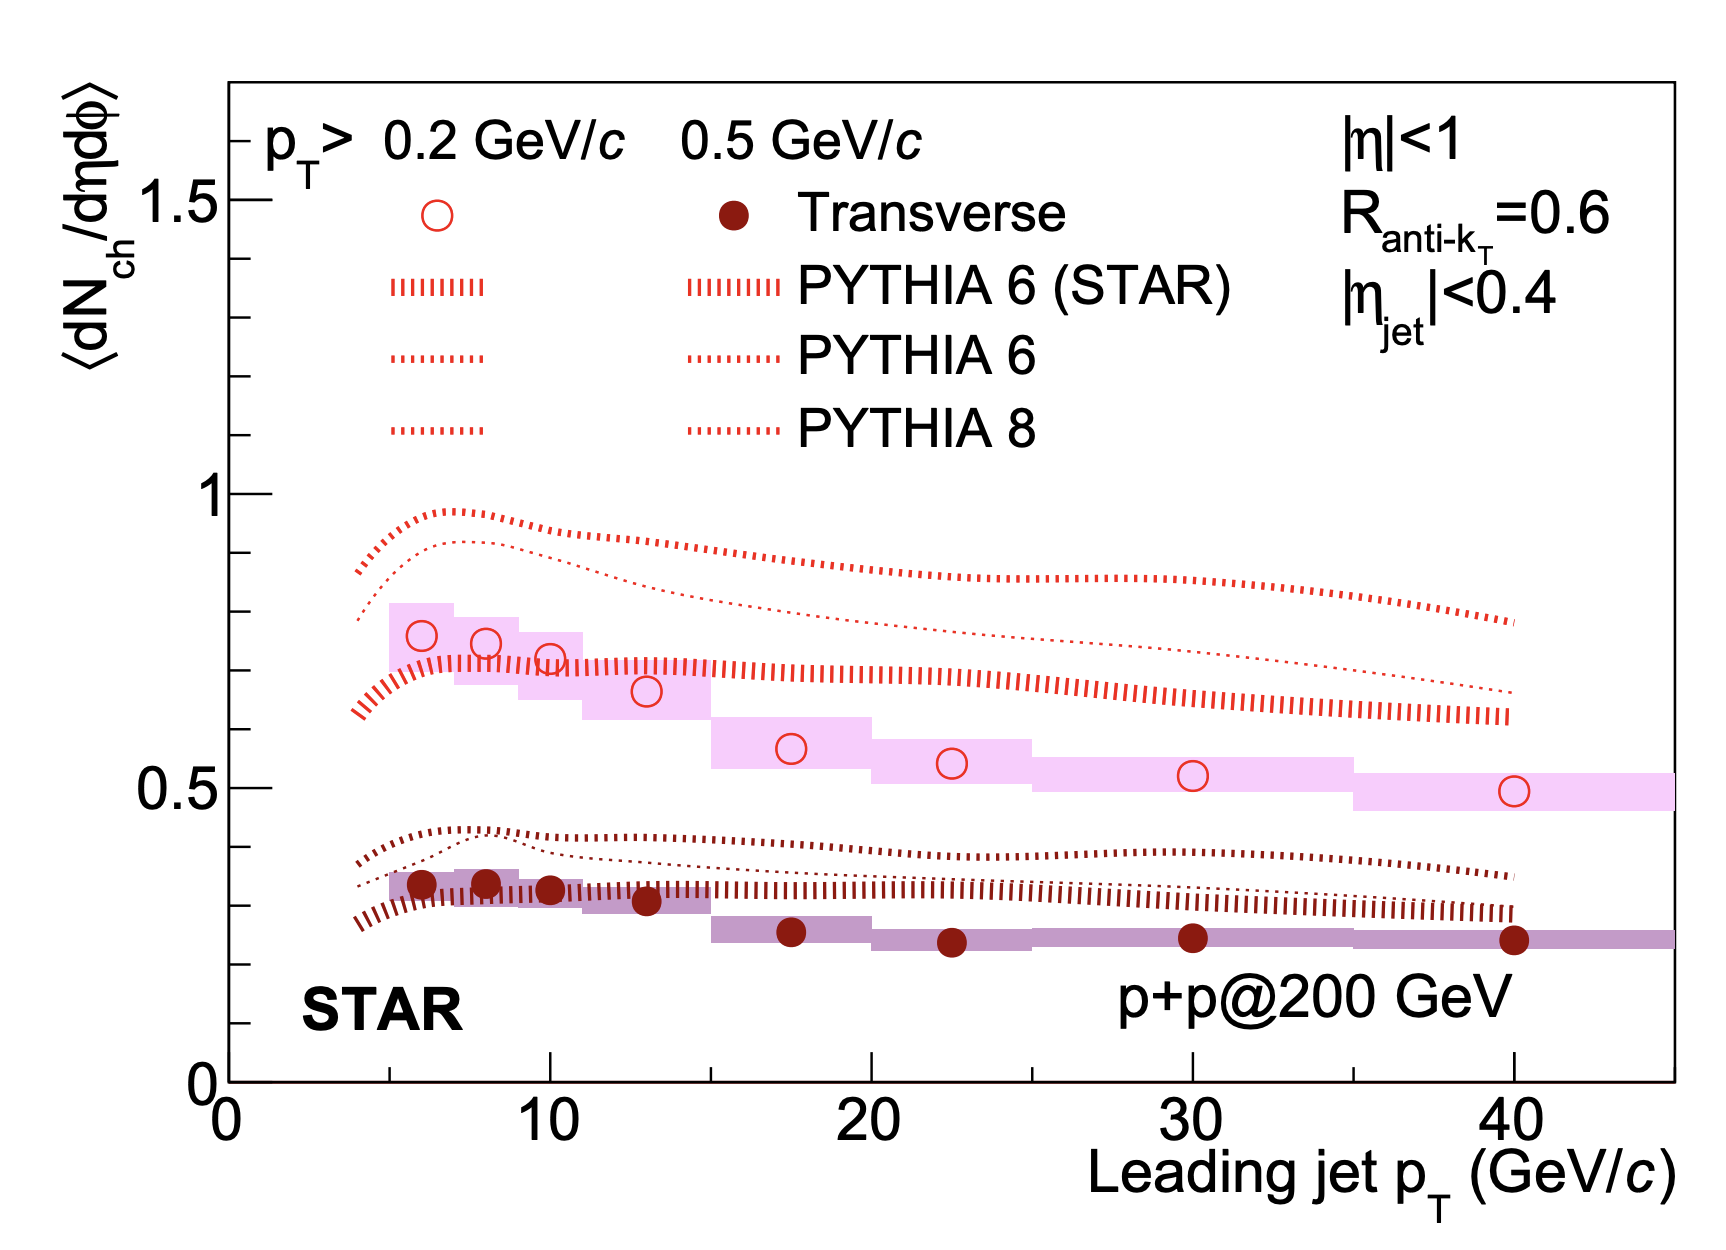
\includegraphics[width=0.7\textwidth]{figures/chapter1/star_ue_in_pp.png}
    \caption{Underlying event measurement in p+p collisions at 200 GeV from STAR. Underlying event as a function of leading jet pT for inclusive jet events is shown for two different charged hadron minimum $p_{T}$ thresholds. Reproduced from~\cite{STAR:2024underlying_event_pp_200gev}.}
    \label{fig:ue_pp_star}
\end{figure}
Results from STAR at RHIC energies of 200 GeV~\cite{STAR:2024underlying_event_pp_200gev} (Figure \ref{fig:ue_pp_star}) show a similar trend to the ATLAS exclusive dijet results, where the UE decreases slightly with increasing leading-jet $p_{T}$.
It is argued that the decrease in the UE with increasing leading-jet $p_{T}$ is consistent with energy conservation behavior, and when the UE is measured on either side of the transverse region, denoted as the TransMax and TransMin regions, the UE is found to be fairly consistent between the two regions. 
This suggests that ISR/FSR contributions which would be more likely to be localized and therefore in only one region of the transverse region are lower at RHIC than at LHC.

\begin{figure}
    \centering
    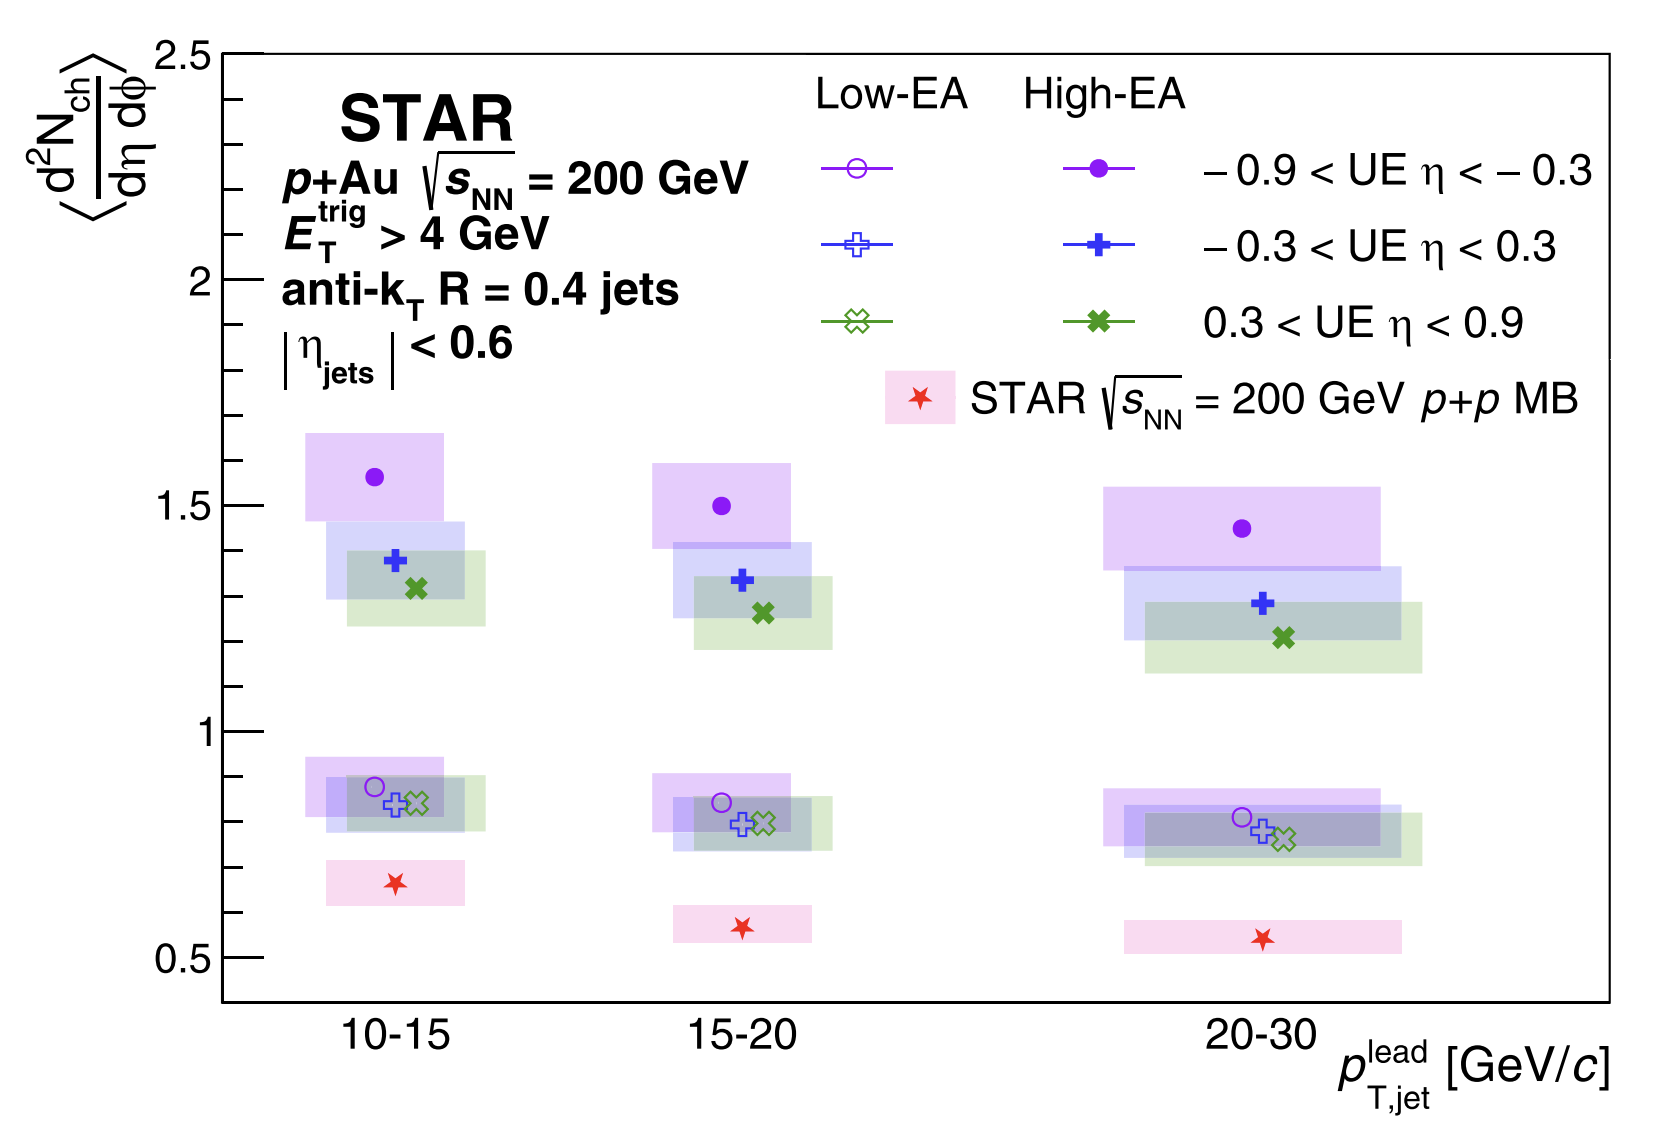
\includegraphics[width=0.7\textwidth]{figures/chapter1/star_ue_in_pAu.png}
    \caption{Underlying event measurements in p+Au collisions at 200 GeV from STAR. Plot shows the underlying event as a function of leading jet pT for dijet events for a selection of events with high- and low-event activity as determined from the forward region. Reproduced from~\cite{star_ue_pAu}.}
    \label{fig:ue_pAu_star}
\end{figure}
Additional studies in proton-Gold collisions at RHIC also use the event shape shown in Figure \ref{fig:UEeventshape} to estimate the underlying event and see a similar trend of an anti-correlation between the leading-jet $p_{T}$ and the underlying event for p+Au events~\cite{star_ue_pAu}.
This anti-correlation is studied in dijets as a function of event activity measured in the forward region and is attributed to parton x or $Q^2$ initial state effects, rather than radiation effects, due to the correlation spanning multiple units of rapidity. 
This indicates that there are initial state effects that cause a bias in the event activity measurement as a function of the hard scattering kinematics, namely the parton x or $Q^2$ of the hard scattering, which could be due to energy conservation or color fluctuations in the proton.

\begin{figure}
    \centering
    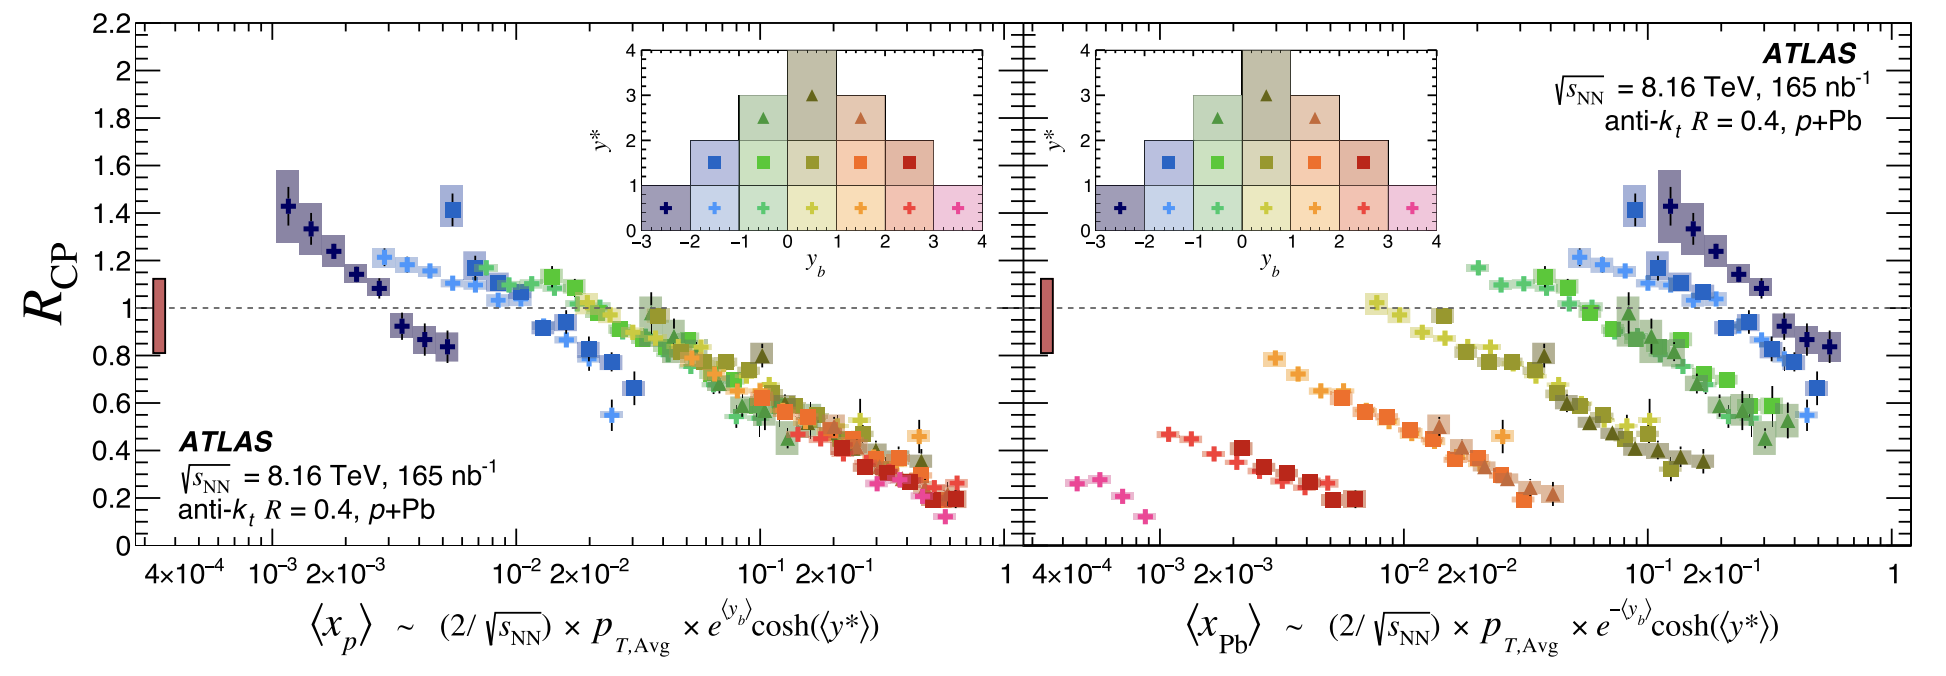
\includegraphics[width=\textwidth]{figures/chapter1/atlas_RpA_dijet.png}
    \caption{Dijet measurements in p+p collisions at 7 TeV from ATLAS. The left plots shows the dijet Rcp as a function of proton parton x, while the right plots shows the dijet Rcp as a function of the lead ion parton x. Reproduced from~\cite{ATLAS:2024dijet_centrality_pPb_816tev}.}
    \label{fig:dijet_pPb_atlas}
\end{figure}
Proton-ion studies at the LHC also see an anti-correlation between the leading-jet $p_{T}$ and the event activity measured in the forward region, which due to the smooth variation as a function of the proton parton x is attributed to initial state effects like color fluctuations in the proton~\cite{ATLAS:2024dijet_centrality_pPb_816tev}.
In particular, the ATLAS measurement of dijets in p+Pb collisions as a function of event activity in the forward region (Figure \ref{fig:dijet_pPb_atlas}) shows a clear trend of suppression of the dijet Rcp at large proton x, which is well explained by color fluctuation effects directly related to small configurations of the proton with reduced interaction strength at high x. 
The suppression in Rcp, the ratio between the yield in central (high event acitivty) and peripheral (low event activity) regions, develops from the correlation between the proton parton x and the total event activity, where at larger proton parton x, it is less likely the collision with have a high event activity, leading to a suppression in Rcp at large proton x.

An additional followup study of the correlation between event activity and hard scattering kinematics in p+p collisions at the LHC was conducted by ATLAS using dijets and event activity measured in the forward region, which also shows a clear anti-correlation between the event activity and the leading jet pT at large jet pT~\cite{ATLAS:2016transverse_energy_pp_276tev}, which is attributed to energy conservation effects, shown in Figure \ref{fig:atlas_dijet_pp_EA_vs_pt}.
However, when studied more differentially, it was found that these energy conservation effects are localized to only the target proton (shown in Figure \ref{fig:atlas_dijet_pp_EA_vs_x}), and are not observed in the projectile proton, indicating that the Rcp suppression observed in p+Pb collisions that scales directly with the proton parton x is not due to energy conservation effects, but rather color fluctuation effects.
\begin{figure}
    \centering
    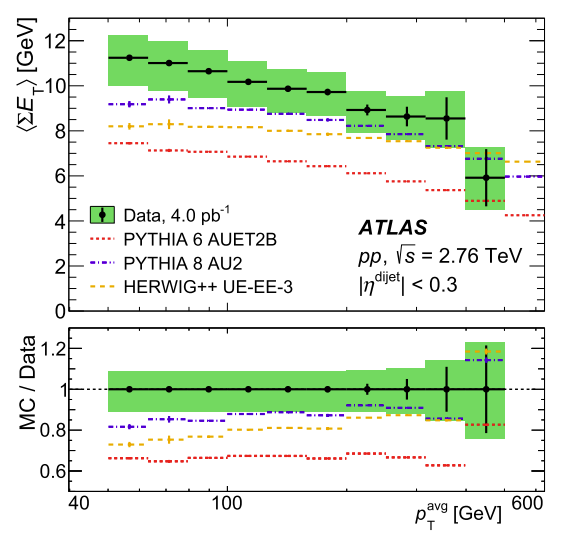
\includegraphics[width=0.7\textwidth]{figures/chapter1/atlas_dijet_pp_EA_vs_pt.png}
    \caption{Underlying event measurements in p+p collisions at 7 TeV from ATLAS. Plot shows the underlying event as a function of leading jet pT for exclusive dijet events for a selection of events with high- and low-event activity as determined from the forward region. Reproduced from~\cite{ATLAS:2016transverse_energy_pp_276tev}.}
    \label{fig:atlas_dijet_pp_EA_vs_pt}
\end{figure}

\begin{figure}
    \centering
    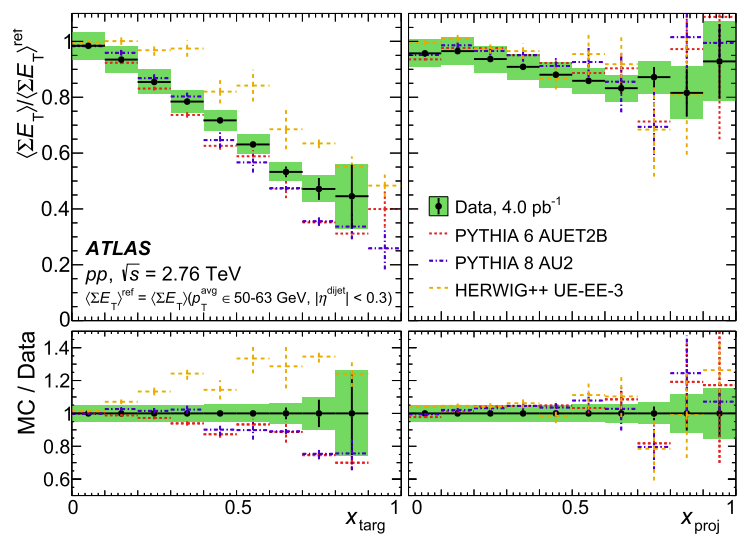
\includegraphics[width=\textwidth]{figures/chapter1/atlas_dijet_pp_EA_vs_x.png}
    \caption{Underlying event measurements in p+p collisions at 7 TeV from ATLAS. Plot shows the underlying event as a function of leading jet pT for exclusive dijet events for a selection of events with high- and low-event activity as determined from the forward region, but plotted as a function of the proton parton x instead of the leading jet pT. Reproduced from~\cite{ATLAS:2016transverse_energy_pp_276tev}.}
    \label{fig:atlas_dijet_pp_EA_vs_x}
\end{figure}
Therefore, there are a number of different initial state effects that could be responsible for the anti-correlation between the leading jet $p_{T}$ and the underlying event observed at RHIC and in exclusive dijet events at the LHC, including energy conservation effects and color fluctuation effects, while the correlation observed in inclusive dijet events at the LHC is likely due to ISR/FSR effects.
Whether the UE observable is sensitive to these initial state effects and not dominated by ISR/FSR effects at RHIC energies is a question this thesis looks to address in part by investigating the UE in p+p collisions at RHIC energies for both inclusive jet events and with an exclusive dijet selection, and by comparing to the UE in p+p collisions at LHC energies for both inclusive jet events and with an exclusive dijet selection.
